\documentclass{article}
\usepackage{tikz}
\usepackage{amsmath}
\usepackage{amsthm}
\usetikzlibrary{calc}
\begin{document}
Elucidations: 
When the legs of an angle are produced or prolonged beyond its vertex, the angles made by them on both ides of the vertex are said to be \textit{vertically opposite} to each other: Thus the red and tellow angles are said to be vertically opposite angles. 

\textit{Superposition} is the process by which one magnitude may be conceived to be placed upon another, so as exavtly to cover it, or so that every part os each shall exactly coincide. 

A line is said to be \textit{produced}, when it is extended, prolonged, or has its length increased, and the increase of length which it receives is called its \textit{produced part}, or its \textit{protrusion}. 

The entire length of the line or lines which enclose a figure, is called its perimeter. The first dix books of Euclid treat of plain figures only. A line drawn from the centre of a circle to its circumference, is called a \textit{radius}. The lines which include a figure are called its \textit{sides}. That side of a right angled triangle, which is opposite to the right angle, is called the \textit{hypotenuse}. An \textit{oblong} is defined in the second book, and called a \textit{recntagle}. All the lines which are considered in the first six books of the Elements are supposed to be in the same plane. 
The \textit{straight-edge} and \textit{compasses} are the only instruments, the use of which is permitted in Euclid, or plain Geometry. To declare this restriction is the object of the \textit{postulates}. 

The \textit{Axioms} of geometry are certain general propositions, the truth of which is taken to be self-evident and incapable of being established by demonstration. 

\textit{Propositions} are those results which are obtained in geometry by a process of reasoning. There are two species of propositions in geometry, \textit{problems} and \textit{theorems}. 

A \textit{Problem} is a proposition in which something is proposed to be done; as a line to be drawn under some given conditions, a circle to be described, some figure to be constructed, \&c. 

The \textit{Solution} of the problem consists in showing how the thing required may be done by the aid of the rule or straight-edge and compasses. 

The \textit{demonstration} consists in proving that the process indicated in the solution really attains the required end. 

A \textit{Theorem} is a proposition in which the truth of some principle is asserted. This principle must be deduced from the axioms and definitions, or other truths previouslu and independently established. To show this is the subject of demonstration. 

A \textit{Problem} is analogous to a postulate. 

A \textit{Theorem} resembles an axiom. 

A \textit{Postulate} is a problem, the solution of which is assumed. 

An \textit{Axiom} is a theorem, the truth os which is granted without demonstration. 

A \textit{Corollary} is an inference deduced immediately from a proposition. 

A \textit{Scholium} is a note or observation on a proposition not containing an inference of sufficient importance to entitle it to the name of \textit{corollary}. 

A \textit{Lemma} is a proposition merely introduced for the purpose of establishing some more important proposition. 

\newcommand{\manydots}[2][9pt]{
\begin{tikzpicture}
\foreach \x in {1,...,#2} 
\fill (\x*#1,0) circle (0.55pt);
\end{tikzpicture}
}

\newcommand{\therefore}{
\begin{tikzpicture}[scale=0.18]
\fill (0,0) circle (5pt);
\fill (1,0) circle (5pt);
\fill (60:1) circle (5pt);
\end{tikzpicture}} 

\newcommand{\because}{
\begin{tikzpicture}[scale=-0.18]
\fill (0,0) circle (5pt);
\fill (1,0) circle (5pt);
\fill (60:1) circle (5pt);
\end{tikzpicture}} 

\newcommand{\equals}{
\ensuremath{
\mathrel{
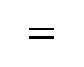
\begin{tikzpicture}[baseline=-0.5ex]
\draw[line width=1.0pt] (0,1.5pt) -- (9pt,1.5pt);
\draw[line width=1.0pt] (0,-1.5pt) -- (9pt,-1.5pt);
\end{tikzpicture}}}
}

\newcommand{\notequals}{
\ensuremath{
\mathrel{
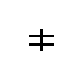
\begin{tikzpicture}[baseline=-0.5ex]
\draw[line width=1.0pt] (0,1.5pt) -- (9pt,1.5pt);
\draw[line width=1.0pt] (0,-1.5pt) -- (9pt,-1.5pt);
\draw[line width=1.0pt] (4.5pt,-4pt) -- (4.5pt,4pt);
\end{tikzpicture}}}
}

\newcommand{\greater}{
\ensuremath{
\mathrel{

\begin{tikzpicture}
\draw[line width=1.0pt] (9pt,2.5pt) -- (0,2.5pt) -- (0,-2.5pt) -- (9pt,-2.5pt);
\end{tikzpicture}}}
}
\newcommand{\less}{
\ensuremath{
\mathrel{
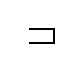
\begin{tikzpicture}[scale=-1]
\draw[line width=1.0pt] (9pt,2.5pt) -- (0,2.5pt) -- (0,-2.5pt) -- (9pt,-2.5pt);
\end{tikzpicture}}}
}
\newcommand{\notgreater}{
\ensuremath{
\mathrel{

\begin{tikzpicture}
\draw[line width=1.0pt] (9pt,2.5pt) -- (0,2.5pt) -- (0,-2.5pt) -- (9pt,-2.5pt);
\draw[line width=1.0pt] (4.5pt,-5pt) -- (4.5pt,5pt);
\end{tikzpicture}}}
}
\newcommand{\notless}{
\ensuremath{
\mathrel{

\begin{tikzpicture}[scale=-1]
\draw[line width=1.0pt] (9pt,2.5pt) -- (0,2.5pt) -- (0,-2.5pt) -- (9pt,-2.5pt);
\draw[line width=1.0pt] (4.5pt,-5pt) -- (4.5pt,5pt);
\end{tikzpicture}}}
}
\newcommand{\plus}{
\ensuremath{
\mathbin{
\begin{tikzpicture}
\draw[line width=1.0pt] (0pt,-4pt) -- (0pt,4pt);
\draw[line width=1.0pt] (-4pt,0pt) -- (4pt,0pt);
\end{tikzpicture}}}
}
\newcommand{\minus}{
\ensuremath{
\mathbin{
\begin{tikzpicture}
\draw[line width=1.0pt] (-4pt,0pt) -- (4pt,0pt);
\end{tikzpicture}}}
}
\newcommand{\cross}{
\ensuremath{
\mathbin{

\begin{tikzpicture}[rotate=45]
\draw[line width=1.0pt] (0pt,-4pt) -- (0pt,4pt);
\draw[line width=1.0pt] (-4pt,0pt) -- (4pt,0pt);
\end{tikzpicture}}}
}
\newcommand{\isto}{
\ensuremath{
\mathrel{
\begin{tikzpicture}
\fill (0,1.5pt) circle (1pt);
\fill (0,-1.5pt) circle (1pt);
\end{tikzpicture}}}
}
\newcommand{\as}{
\ensuremath{
\mathrel{

\begin{tikzpicture}
\fill (-1.5pt,1.5pt) circle (1pt);
\fill (-1.5pt,-1.5pt) circle (1pt);
\fill (1.5pt,1.5pt) circle (1pt);
\fill (1.5pt,-1.5pt) circle (1pt);
\end{tikzpicture}}}
}

\newcommand{\plel}{
\ensuremath{
\mathrel{

\begin{tikzpicture}
\draw[line width=1pt] (-1.2pt,-4.0pt) -- (-1.2pt,4.0pt);
\draw[line width=1pt] (1.2pt,-4.0pt) -- (1.2pt,4.0pt);
\end{tikzpicture}}}
}
\newcommand{\perpendicular}{
\ensuremath{
\mathrel{
\begin{tikzpicture}
\draw[line width=1pt] (0pt,6.0pt) -- (0pt,0pt);
\draw[line width=1pt] (-4.0pt,0pt) -- (4.0pt,0pt);
\end{tikzpicture}}}
}

\newcommand{\acuteangle}{
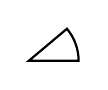
\begin{tikzpicture}[thick]
\draw (0,0) -- (18pt,0) arc (0:40:18pt) -- cycle;
\end{tikzpicture}
}
\newcommand{\rightangle}{

\begin{tikzpicture}[thick]
\draw (0,0) -- (18pt,0) arc (0:90:18pt) -- cycle;
\end{tikzpicture}
}
\newcommand{\rightangles}{
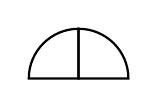
\begin{tikzpicture}[thick]
\draw (0,0) -- (18pt,0) arc (0:90:18pt) -- cycle;
\draw (0,0) -- (0,18pt) arc (90:180:18pt) -- cycle;
\end{tikzpicture}
}
\newcommand{\vertex}{

\begin{tikzpicture}[scale=0.35,ultra thick,rotate=-93]
\draw (0,0) -- (1,0) -- (0,0) -- (40:1);
\end{tikzpicture}
}
\newcommand{\trivertex}{

\begin{tikzpicture}[scale=0.6,ultra thick,rotate=-130]
\clip[rotate=130] (-1,-0.6) rectangle (0.7,0.1);
\draw (90:1) -- (0,0) -- (1,0);
\draw (1,0) -- (0,0) -- (90:1);
\draw (0,0) -- (40:1);
\end{tikzpicture}
}

\begin{itemize}
\item[\therefore] expresses the word \textit{therefore}.
\item[\because] \manydots{10} \textit{because}.
\item[\equals] \manydots{10} \textit{equal}. This sign of equality may be read \textit{equal to}, or \textit{is equal to}, or \textit{are equal to}; but any discrepancy in regard to the introduction of the auxilliary verys \textit{is,are,}\&c. cannot affect the geometrical rigour. 
\item[\notequals] means the same as if the words ``not equal'' were written.\item[\greater] signifies \textit{greater than}.
\item[\less] \manydots{4} \textit{less than}.
\item[\notgreater]\manydots{4} \textit{not greater than}.
\item[\notless]\manydots{4} \textit{not less than}. 
\item[\plus] is read \textit{plus} (\textit{more}), the sign of addition; and when placed between two magnitudes, signifies their sum. 
\item[\minus] is read \textit{minus} (\textit{less}), signifies subtraction; and when placed between two quantities denotes that the latter is to be taken from the former. 
\item[\cross] this sign expresses the product of two or more numbers when placed between them in arithmetic and algebra; but in geometry it is generally used to express a \textit{rectangle}, when placed between ``two straight lines which contain one of its right angles.'' A \textit{rectangle} may also be represented by placing a point between two of its counterminous sides. 
\item[\isto \as \isto] expresses an \textit{analogy} or \textit{proportion}; thus, if A, B, C and D, represent four magnitudes, and A has to B the same ratio that C has to D, the proposition is thus breifly written 
\begin{align*}
A \isto B &\as C \isto D,\\
A \isto B &\equals C \isto D,\\
\text{or } \frac{A}{B} &\equals \frac{C}{D}
\end{align*}
This equality or sameness of ratio is read 
\begin{center}
as A is to B, so C is to D; \\
or A is to B, as C is to D.
\end{center}
\item[\plel] signifies \textit{parallel} to. 
\item[\perpendicular] \manydots{4} \textit{perpendicular to}.
\item[\acuteangle] \manydots{1} \textit{angle}.
\item[\rightangle] \manydots{2} \textit{right angle}.
\item[\rightangles] \textit{two right angles}. 
\item[\trivertex or \vertex] briefly designates a \textit{point}.
\item[\greater,\equals or \less] signifies \textit{greater, equal, or less than}. 
\item[] The square described on a line is concisely written thus, ${\tikz[ultra thick,baseline=-0.5ex] \draw (0,0) -- (1,0);}^{2}$
\item[] In the same manner twice the square of, is expressed by $2 \cdot{\tikz[ultra thick,baseline=-0.5ex] \draw (0,0) -- (1,0);}^{2}$
\item[def.] signifies \textit{definition}.
\item[pos.] \manydots{4} \textit{postulate}.
\item[ax.] \manydots{4} \textit{axiom}.
\item[hyp.] \manydots{4} \textit{hypothesis}. It may be necessary here to remark, that the \textit{hypothesis} is the condition assumed or taken for gtanted. Thus, the hypothesis of the proposition given in the Introduction, is that the triangle is isosceles, or that its legs are equal. 
\item[const.] \manydots{4} \textit{construction}. The \textit{construction} is the change made in the original figure, by drawing lines, making angles, describing circle, \&c. om prder to adapt it to the argument of the demonstration or the solution of the problem. The conditions under which these changes are made, are as indisputable as those contained in the hypothesis. For instance, if we make an angle equal to a given angle, these two angles are equal by construction. 
\item[\qedsymbol]
\begin{tabular}[t]{ll}
\manydots{4}& \textit{Quod erat demonstratum}. \\ &Which was to be demonstrated. 
\end{tabular}
\end{itemize}
\end{document}
